% ============================================================================
% ЧАСТЬ 1. Система радиочастотной идентификации
% ============================================================================
\section{Распределенная система радиочастотной идентификации транспорта}
\begin{frame}[plain, noframenumbering]
    \begin{center}
        \Huge
        Распределенная система радиочастотной идентификации транспорта
    \end{center}
\end{frame}

\begin{frame}[allowframebreaks]
    \frametitle{Система радиочастотной идентификации}
    \begin{center}
        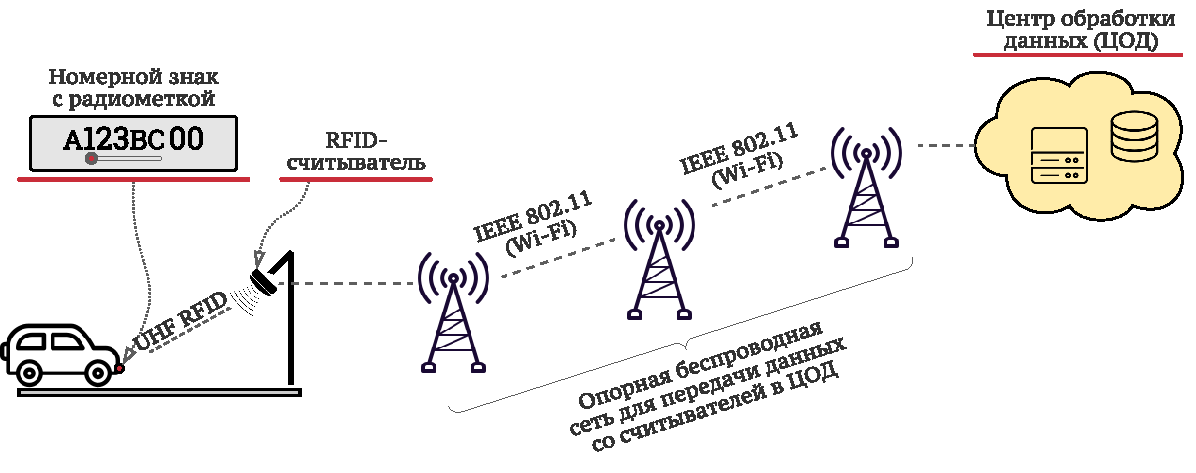
\includegraphics[width=0.9\linewidth]{chapter1/ch1_system_overview}
    \end{center}
    Система радиочастотной идентификации транспорта предназначена для
    идентификации транспорта с помощью размещенных на машинах RFID-меток
    и передачи данных по сети в центр обработки данных. Области применения:
    \begin{itemize}
        \item Повышение безопасности на дорогах "--- надежная идентификация нарушителей, поиск угнанных автомобилей
        \item Бесконтактная оплата проезда по платным дорогам
        \item Контроль доступа, оплата парковки и другие применения
    \end{itemize}
    \vfill
    \framebreak
    \begin{center}
        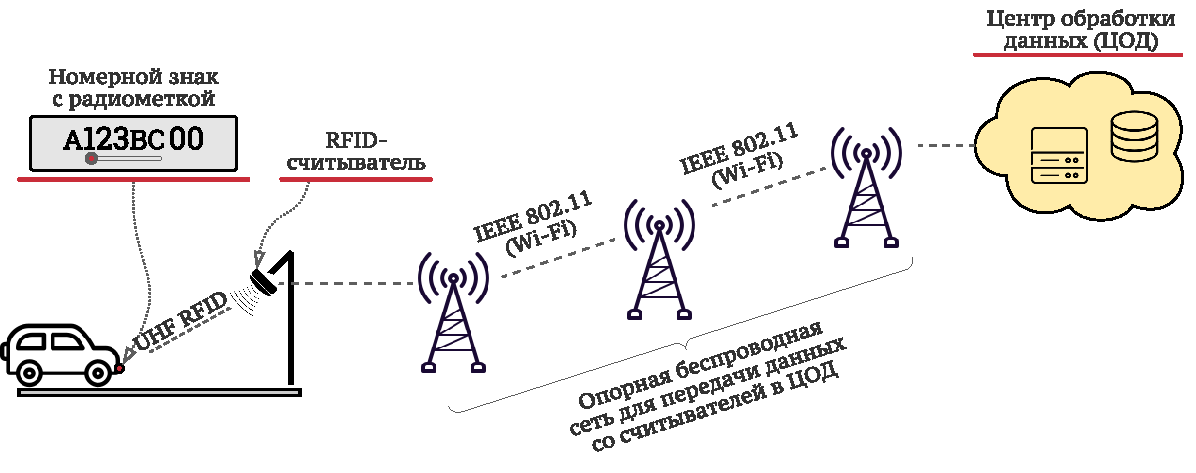
\includegraphics[width=0.9\linewidth]{chapter1/ch1_system_overview}
    \end{center}
    Система включает в себя следующие основные компоненты:
    \begin{itemize}
        \item Пассивные RFID-метки, устанавлиаемые в номера автомобилей
        \item RFID-считыватели, считывающие идентификаторы меток
        \item Сеть передачи
        \item Центр обработки данных
        \item Распределенная компьютерная система управления и сбора данных с RFID-считывателей
    \end{itemize}
\end{frame}
\note{
    Этот текст будет виден только если его отображение включено
    в~файле \textbf{Presentation/setup}.
    Для раздельного вывода презентации и заметок на~разные экраны (как
    в~impress или powerpoint) можно использовать программу
    \textit{pdf-presenter-console}.
}

\begin{frame}
    \frametitle{Постановка задач исследования}
    \begin{enumerate}
        \item Разработка и исследование комплекса аналитических и имитационных моделей для анализа и оптимизации основных характеристик систем радиочастотной идентификации транспортных средств.
        \item Разработка методики оценки производительности широкополосных беспроводных сетей, использующихся для передачи данных от RFID-считывателей в центры обработки данных, на основе методов теории массового обслуживания и марковских случайных процессов.
        \item Разработка архитектуры и реализация распределенной системы управления и сбора данных с RFID-считывателей, ее экспериментальное внедрение и проведение испытаний.
    \end{enumerate}
\end{frame}



% ============================================================================
% ЧАСТЬ 2. ИССЛЕДОВАНИЕ ПРОИЗВОДИТЕЛЬНОСТИ СИСТЕМ РАДИОЧАСТОТНОЙ ИДЕНТИФИКАЦИИ
% ============================================================================
\section{Исследование производительности систем радиочастотной идентификации}
\begin{frame}[plain, noframenumbering]
    \begin{center}
        \Huge
        Исследование производительности систем радиочастотной идентификации
    \end{center}
\end{frame}

\begin{frame}
    \frametitle{Структура системы}
    \vfill
    \begin{minipage}{0.55\linewidth}
        \begin{center}
            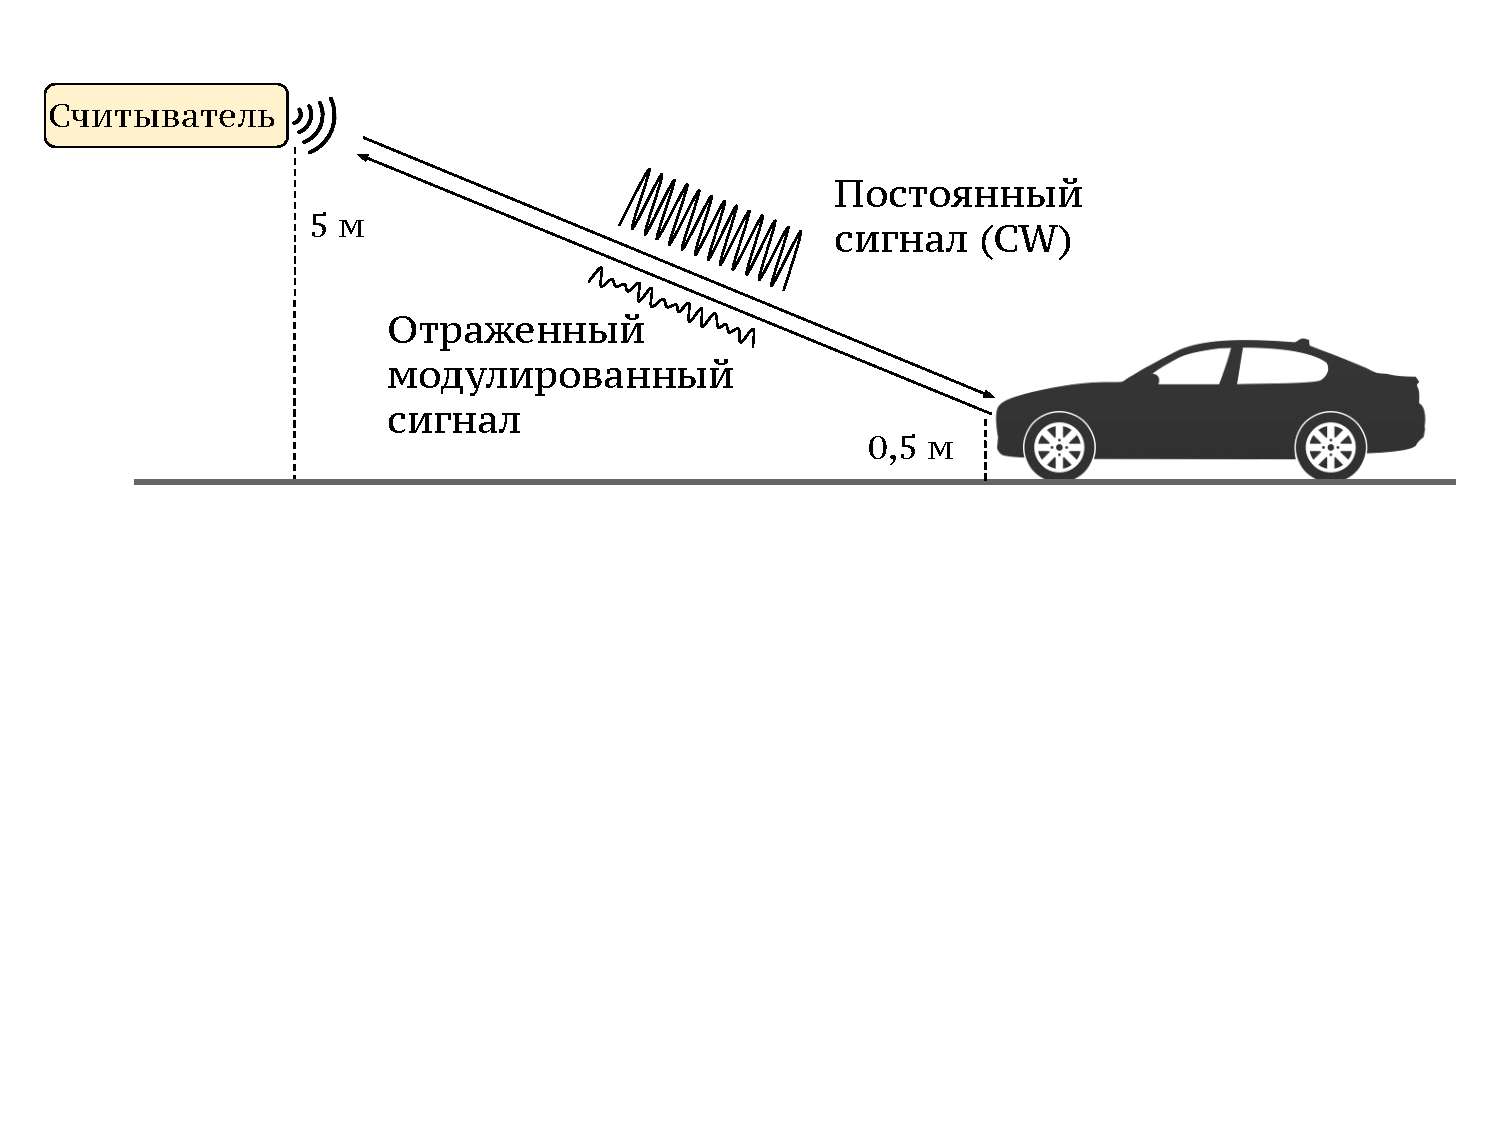
\includegraphics [scale=0.25] {chapter2/ch2_system_structure}
        \end{center}
        Между считывателем и меткой используется протокол международного стандарта EPC Class 1 Gen.2 (ISO 18006-C), диапазон 860 -- 960 МГц.
    \end{minipage}
    \hfill
    \begin{minipage}{0.4\linewidth}
        \begin{itemize}
            \item \textbf{RFID-считыватель}: создает электромагнитное поле, считывает данные с меток
            \item \textbf{Пассивные RFID-метки}: работают в области действия считывателя, передают идентификаторы
        \end{itemize}
    \end{minipage}
    \vfill
\end{frame}

\begin{frame}
    \frametitle{Вероятность идентификации метки}
    Вероятность идентификации RFID-метки на автомобиле можно оценить как:
    \[
        P_t \approx 1 - \left( 1 - (1 - 2^{-Q})^{N_t-1} (1 - p_e)^B \right)^{N_r},
    \]
    где
    \begin{itemize}
        \item $2^Q$ "--- число слотов в раунде опроса
        \item $N_t$ "--- среднее число меток, принимающих участие в раунде
        \item $p_e$ "--- средняя вероятность битовой ошибки (BER)
        \item $B$ "--- общее число бит в ответах метки
        \item $N_r = L / (v \tau)$ "--- среднее число раундов, в которых успевает принять метка, $L$ "--- средняя длина отрезка дороги, на котором метка получает достаточно энергии, $v$ "--- скорость движения метки, а $\tau$ "--- средняя длительность раунда инвентаризации
    \end{itemize}
    Реальное значение BER $p_e(t)$, как и величина $L$, меняются со временем, так как из-за эффекта Доплера канал оказывается зависимым от времени.
\end{frame}


\begin{frame}[allowframebreaks]
    \frametitle{Моделирование радиоканала}
    \vfill
    \begin{center}
        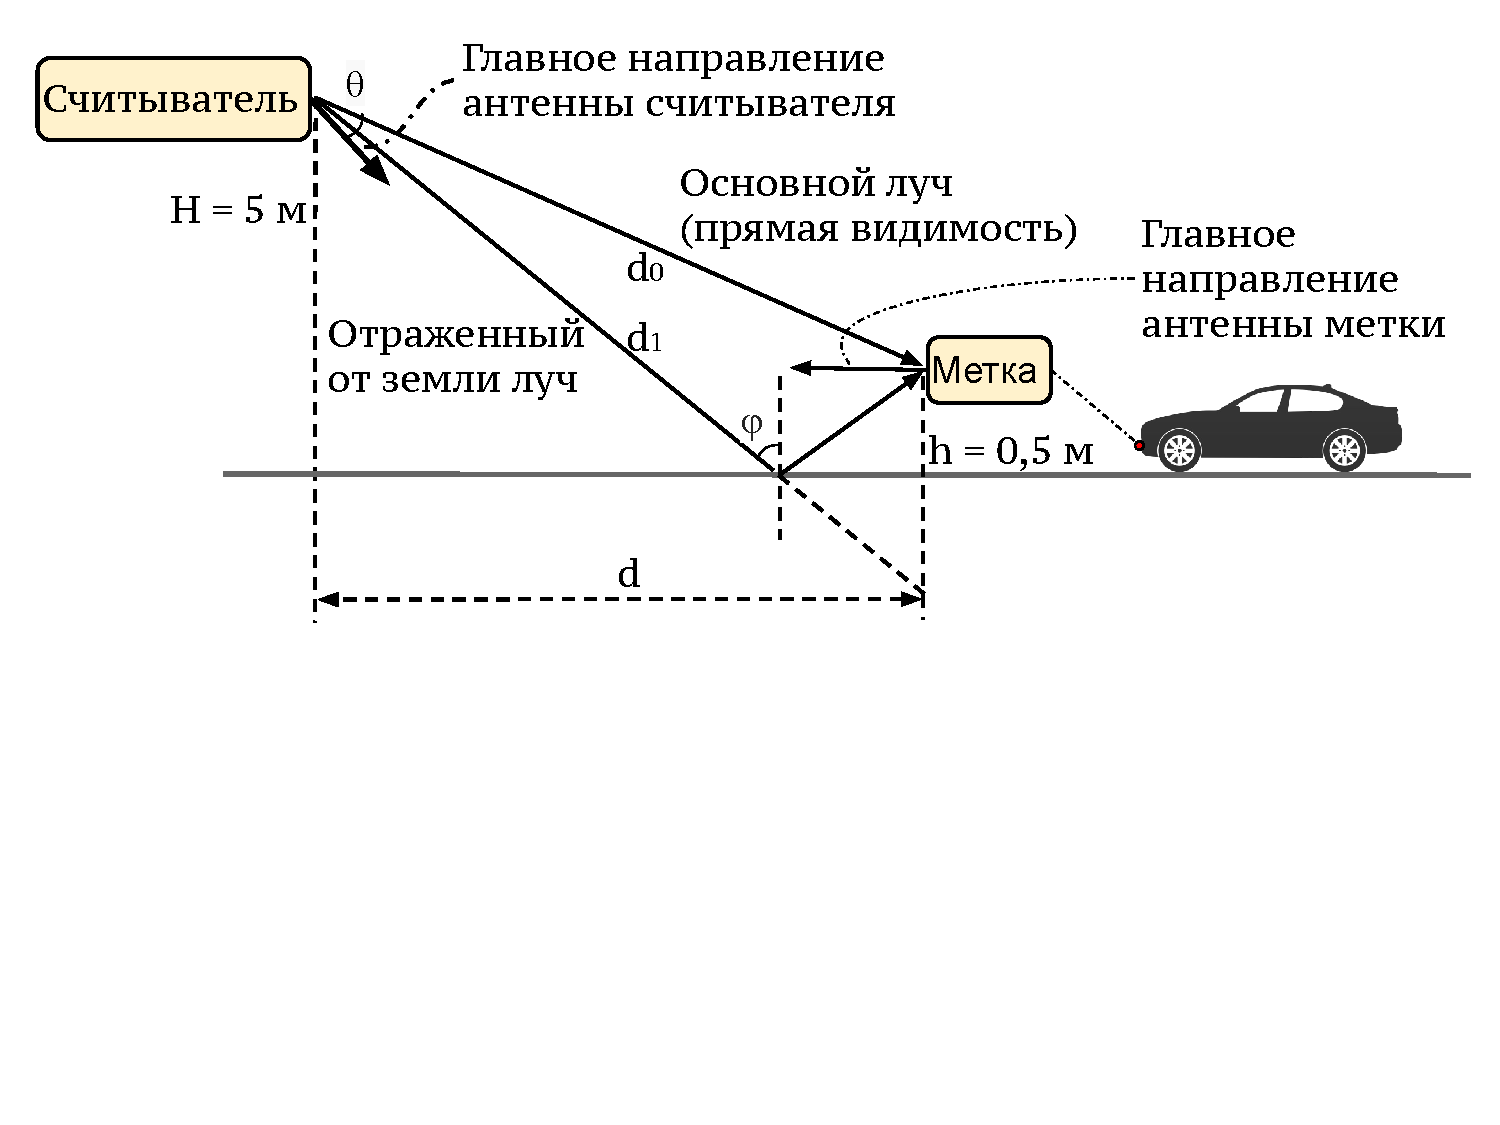
\includegraphics[width=0.8\textwidth]{chapter2/ch2_geometry}
    \end{center}
    Мощность принятого меткой сигнала считывателя:
    $$
        P_r^{(t)} = P_t^{(r)} G^{(r)} A_{pl}^{(d)} A_{pol} G^{(t)}.
    $$
    Мощность принятого считывателем отраженного сигнала:
    $$
        P_r^{(r)} = P_r^{(t)} G^{(t)} A_{bs} A_{pl}^{(r)} A_{pol} G^{(r)}.
    $$
    \vfill
    \framebreak
    \vfill
    \begin{center}
        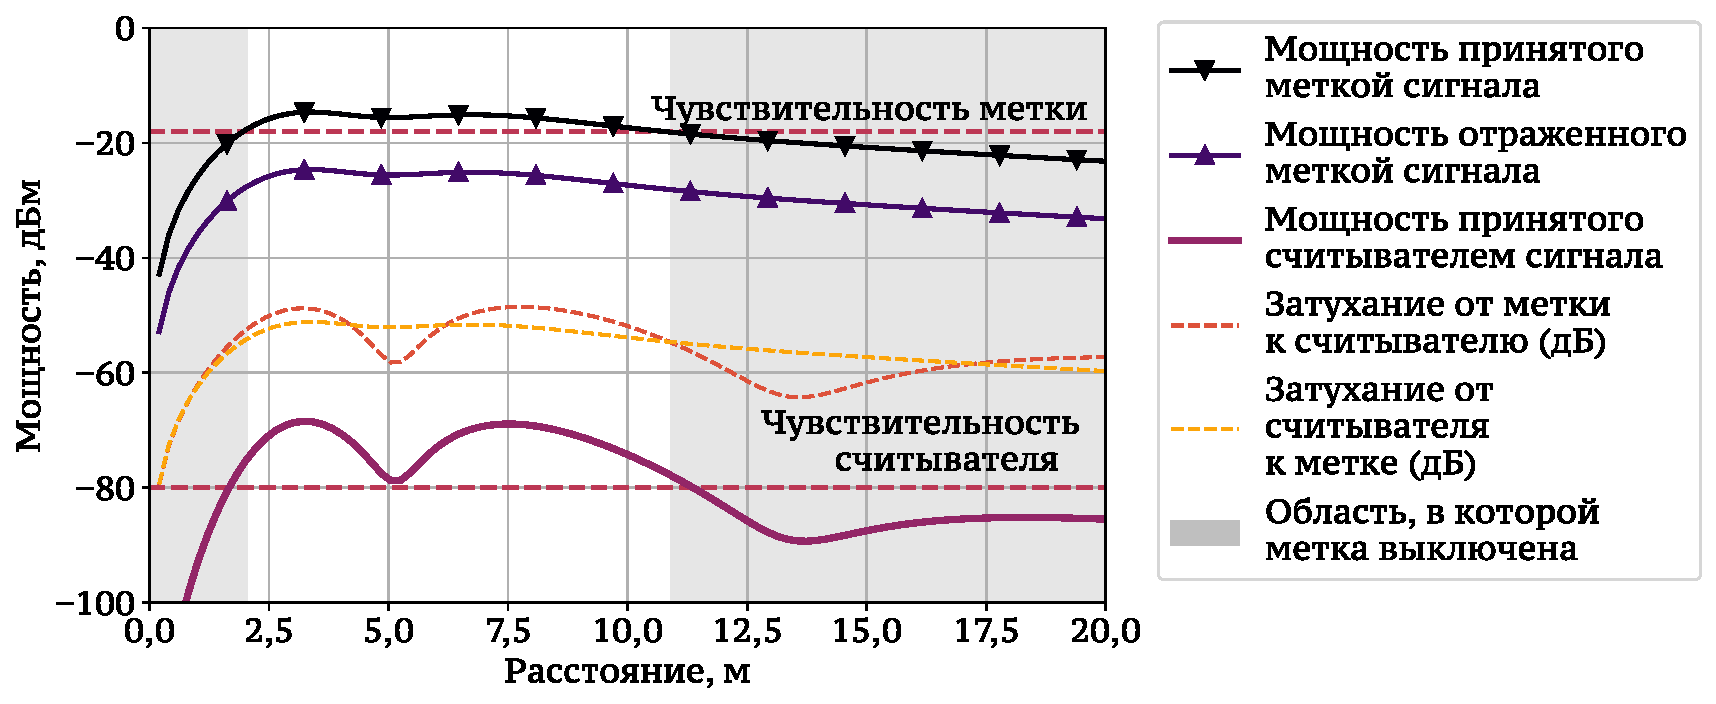
\includegraphics[width=0.99\textwidth]{chapter2/ch2_link_budget}
    \end{center}
    Затухание в канале с многолучевым распространением:
    $$
        A_{pl} = |r(t)|^2 = \left(\frac{\lambda}{4\pi}\right)^2
            \left|\sum\limits_{i=0}^{N} \frac{R_i\Gamma_i}{d_i}
            e^{-jk(d_i-\upsilon t \cos{\psi_i})}\right|^2
    $$
    \vfill
    \framebreak
    \vfill
    \begin{center}
        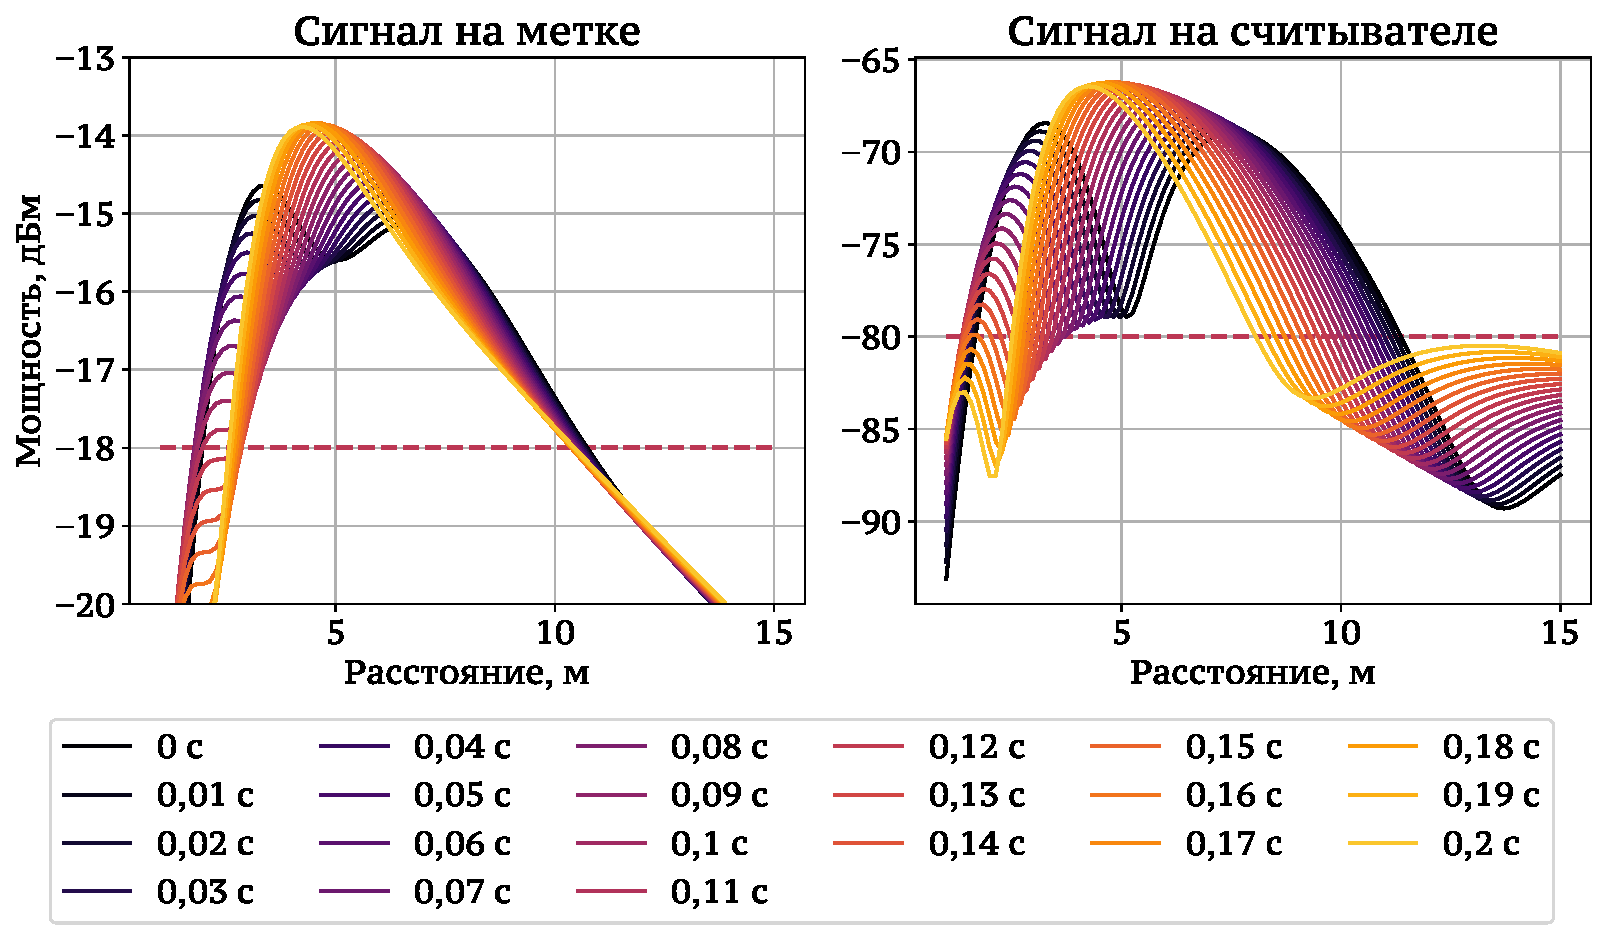
\includegraphics[width=0.99\textwidth]{chapter2/ch2_rx_power_doppler}
    \end{center}
    Существенное влияние на мощность отраженных меткой и принятых считывателем сигналов оказывает эффект Доплера.
    \vfill
  \end{frame}

% \begin{frame}[allowframebreaks]
\begin{frame}
    \frametitle{Расчет вероятности битовой ошибки (BER)}
    \begin{center}
        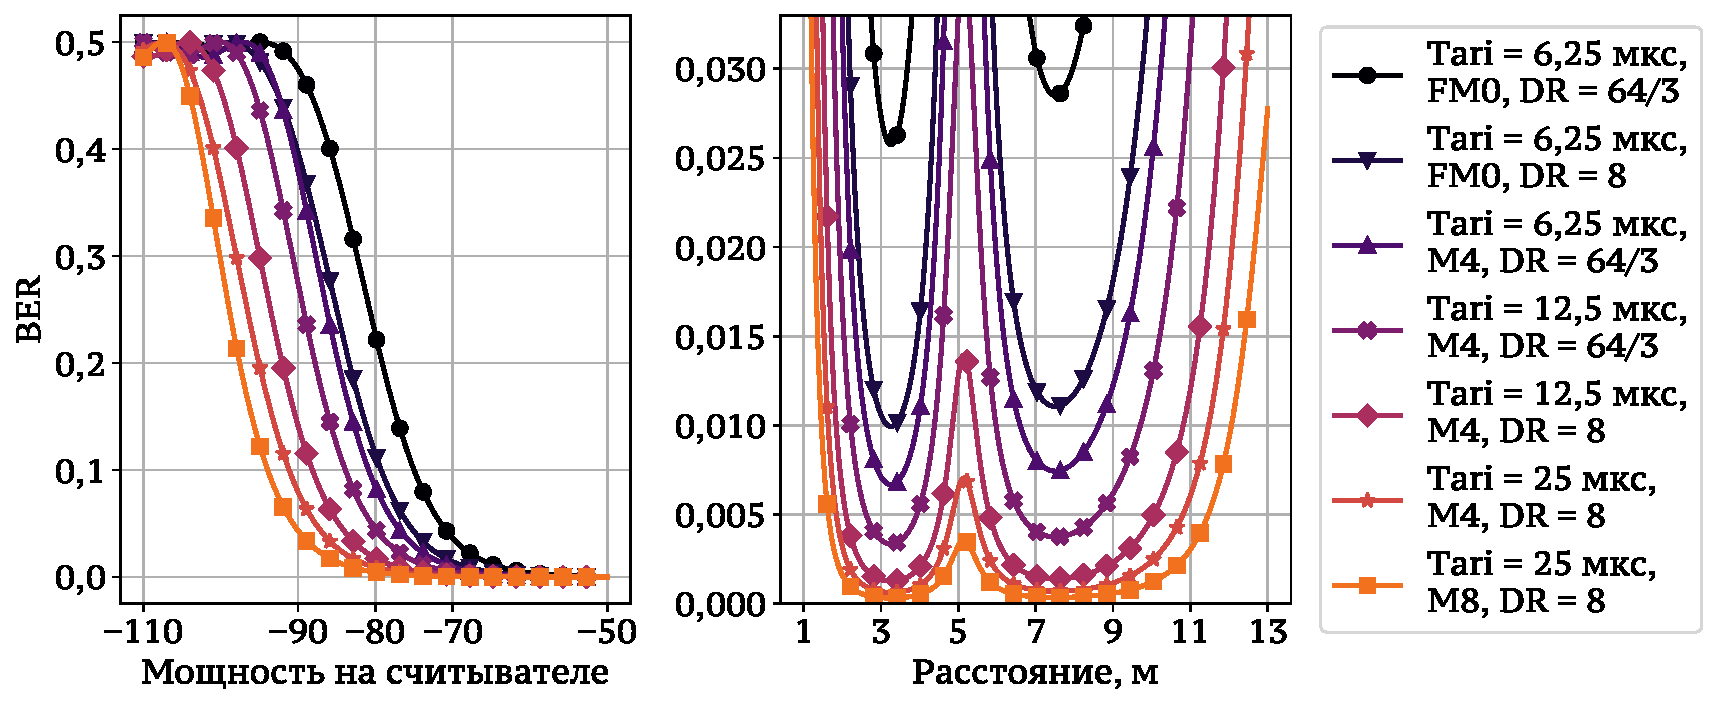
\includegraphics[width=0.9\textwidth]{chapter2/ch2_ber}
    \end{center}
    $$
	    P_{er} = \frac{1}{2} - \frac{1}{\sqrt{1+\frac{2}{\acute{\gamma}}}} +
		    	 \frac{2}{\pi}\frac{\arctan{\sqrt{1+\frac{2}{\acute{\gamma}}}}}{1+\frac{2}{\acute{\gamma}}},
    $$
    где $\acute{\gamma} = mE_s/N_0\cos^2{\phi_s}$; $m$ "--- число символов на бит (порядок) в коде Миллера, $E_s$ "--- энергия одного символа, $N_0/2$ "--- спектральная плотность белого шума и $\phi_s$ "--- разность между реальной и принятой фазами сигнала
    \vfill
    % \framebreak
    % \vfill
    % \begin{center}
    %     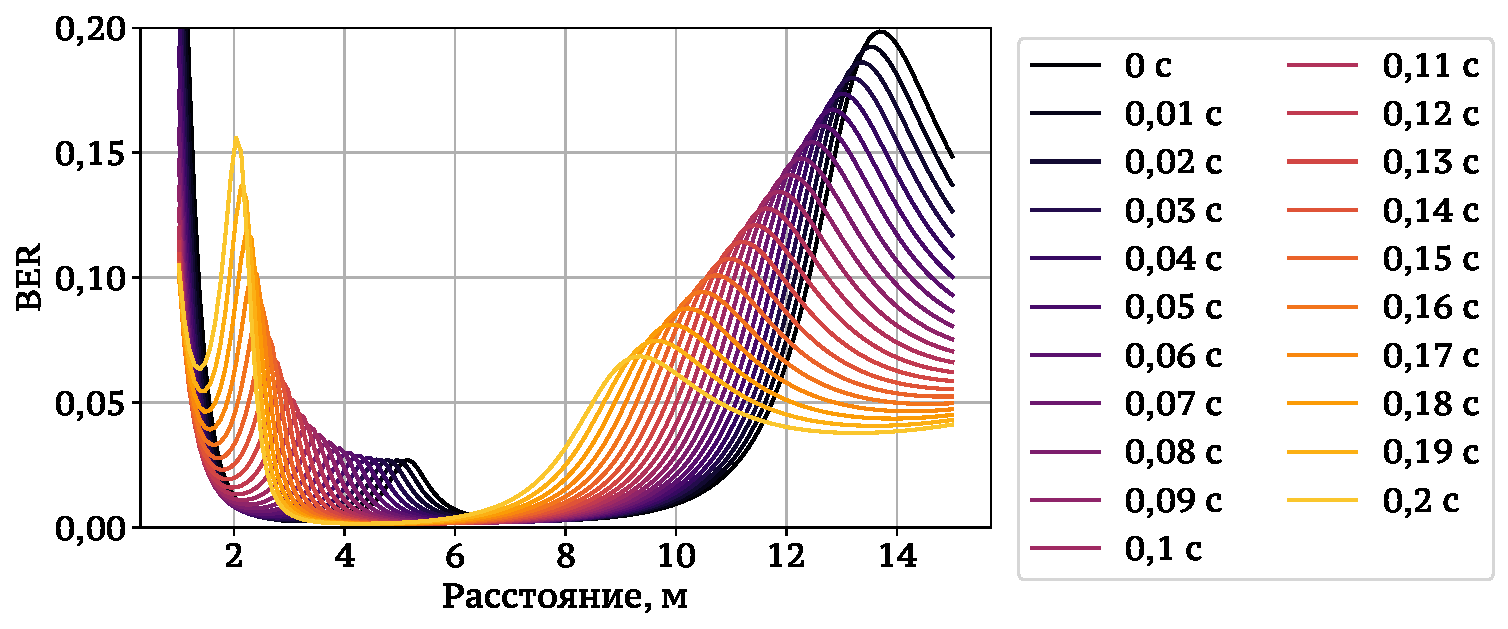
\includegraphics[width=0.99\textwidth]{chapter2/ch2_ber_doppler.pdf}
    % \end{center}
    % Существенное влияние на BER оказывает эффект Доплера.
\end{frame}


\begin{frame}
    \frametitle{Оценка максимального числа раундов опроса}
    \begin{center}
        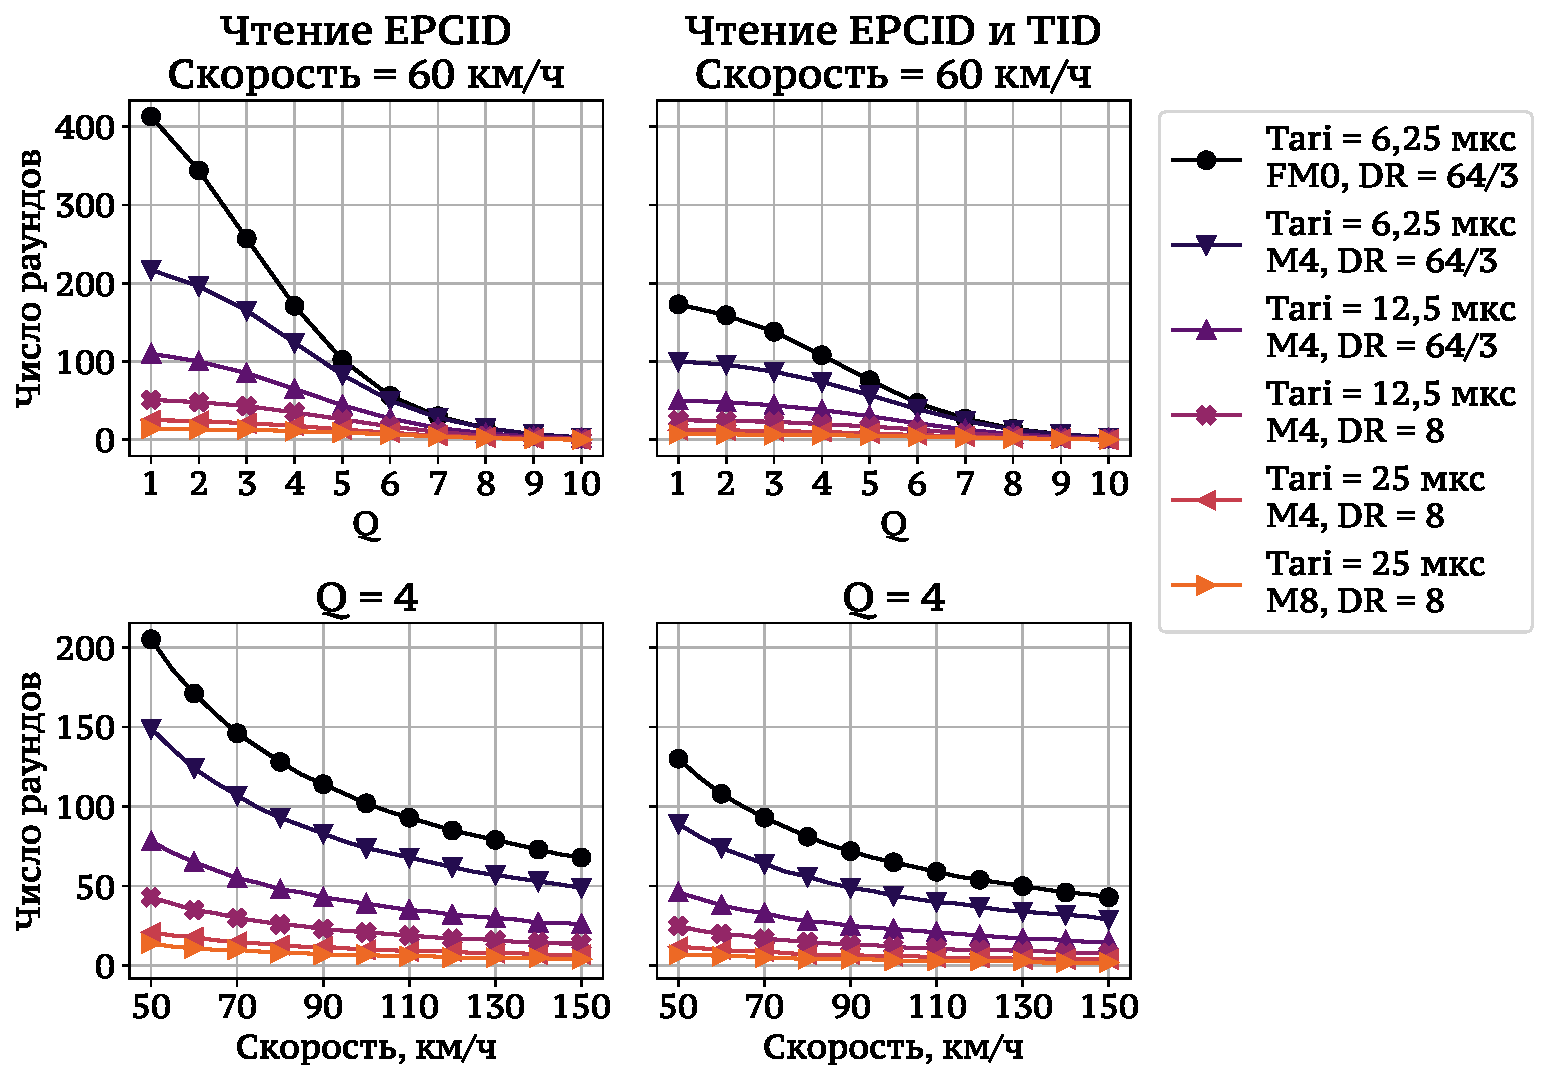
\includegraphics[width=0.8\textwidth]{chapter2/ch2_max_num_rounds.pdf}
    \end{center}
    Длительности команд и ответов существенно зависят от выбранных параметров протокола Tari, M, DR. Из-за этого число раундов опроса, в которых метка может принять участие, может меняться в очень широком диапазоне.
\end{frame}

\begin{frame}
    \frametitle{Имитационная модель системы радиочастотной идентификации}
    Для получения численных результатов при различных настройках считывателей и параметрах окружения была разработана имитационная дискретно-событийная модель. Особенности:

    \begin{itemize}
        \item точный расчет длительности команд, учитывающий кодирование PIE;
        \item учет изменения BER в течение передачи ответов;
        \item моделирование периодических отключений считывателя;
        \item поддержка произвольного числа полос движения и направлений антенн;
        \item учет стратегии выбора флагов сессий для опроса меток;
        \item сбор и анализ различных показателей модели: вероятности идентификации меток, число раундов опроса, в которых учасвует метка, число меток в раундах опроса.
    \end{itemize}

    Модель реализована на языке Python 3, открытый исходный код: \url{https://github.com/larioandr/thesis-rfidsim}
\end{frame}

\begin{frame}
    \frametitle{Результаты: число раундов}
    \begin{center}
        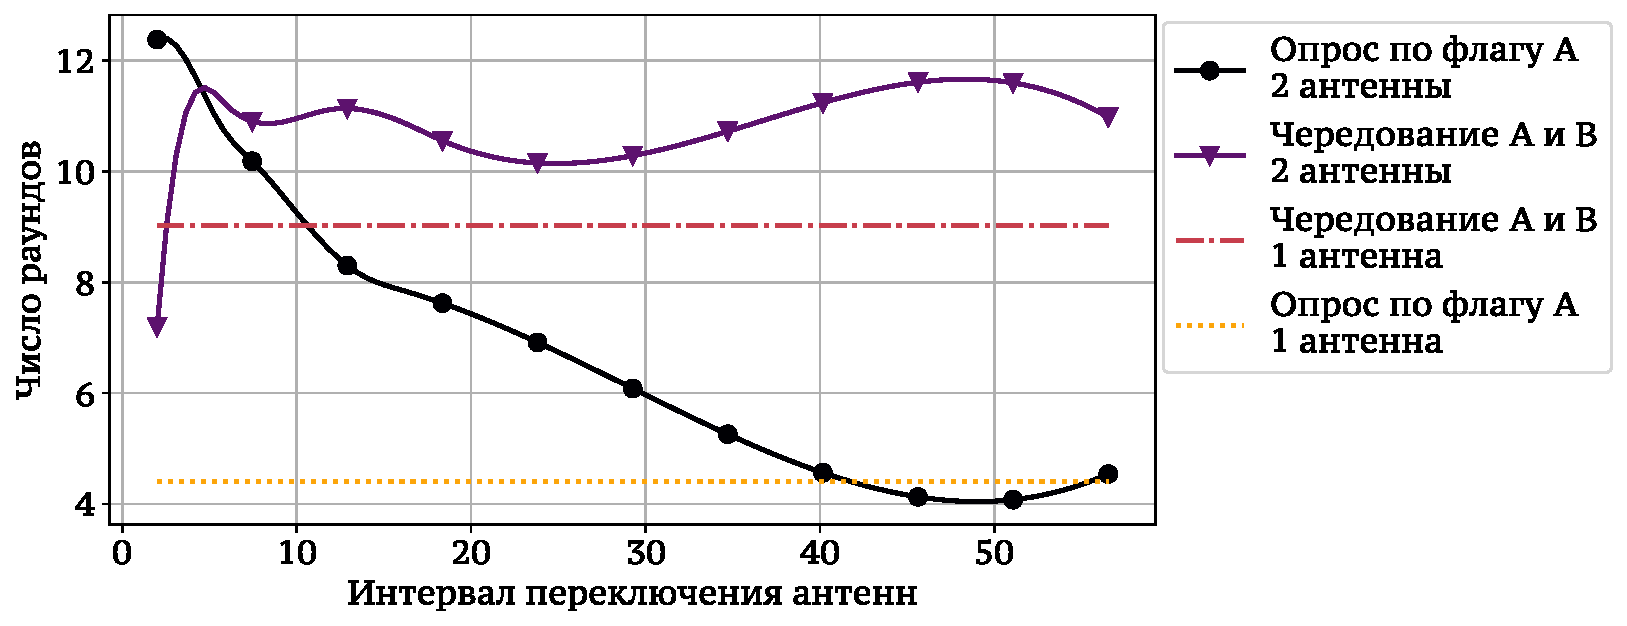
\includegraphics[width=0.9\textwidth]{chapter2/ch2_sim_num_rounds_one_lane}
    \end{center}
    \begin{itemize}
    \item При передаче EPCID метками часто происходят ошибки, из-за инверсии флага сессии метки не могут повторно принять участие в опросе до выключения.
    \item При переключении считывателем антенн часть меток выключается, что ведет к сбросу флага сессии.
    \item Чередование опрашиваемых флагов сессии позволяет эффективно повысить число раундов, в которых метка принимает участие.
    \end{itemize}
\end{frame}

\begin{frame}
    \frametitle{Влияние выбора Tari на вероятность идентификации}
    \begin{center}
        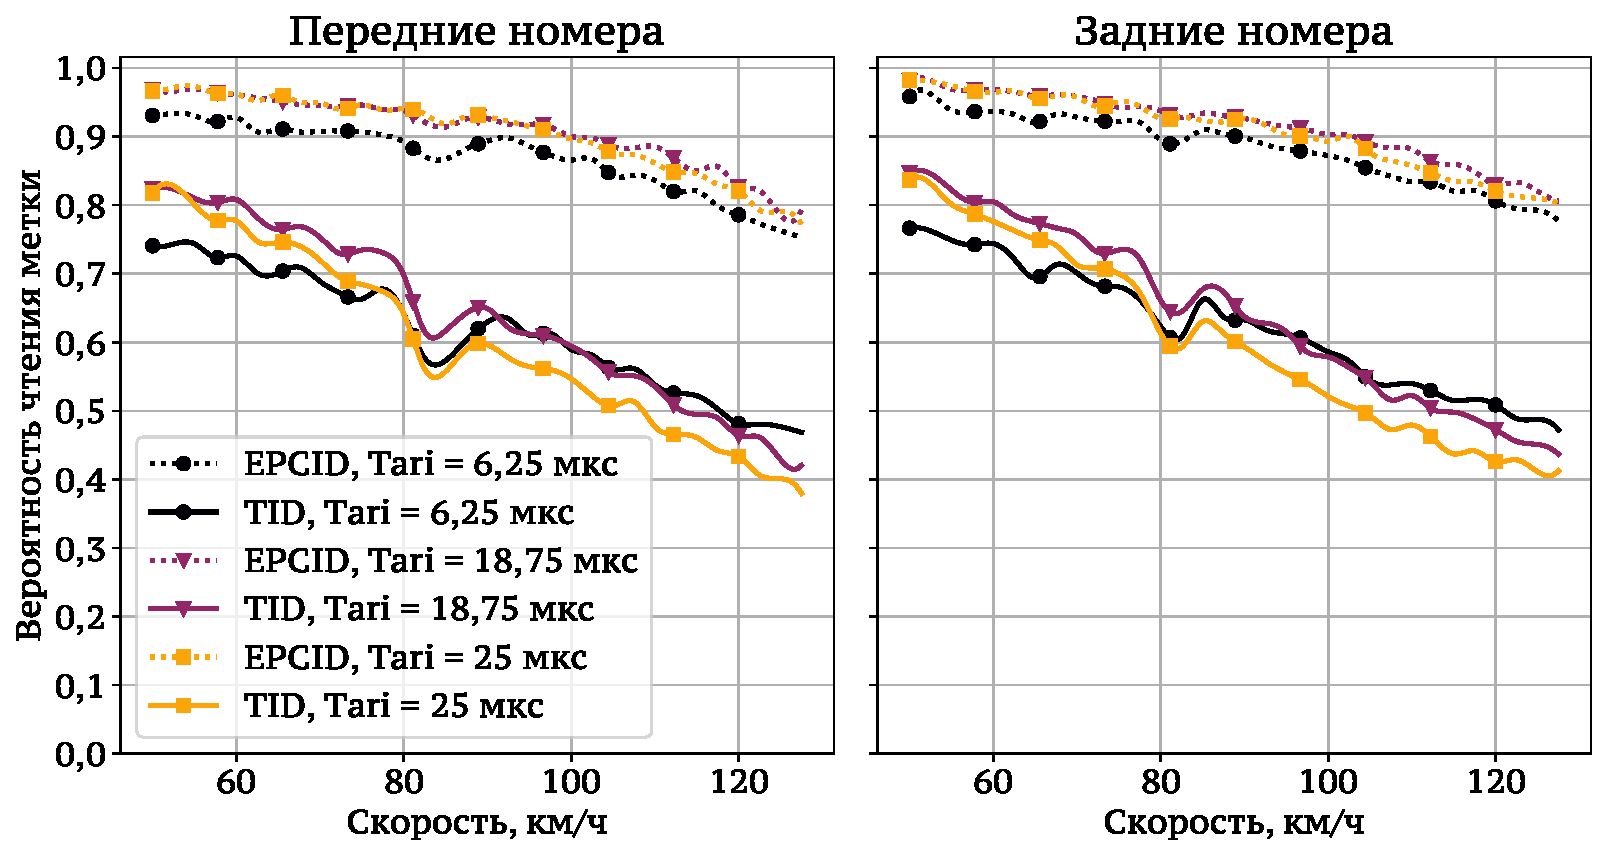
\includegraphics[width=0.8\textwidth]{chapter2/ch2_tag_identification_m4}
    \end{center}
    На графике "--- вероятности идентификации меток при M = 4.
    \begin{itemize}
    \item При низкой скорости эффективнее использовать длинные символы в командах считывателя (Tari = 18,75~мкс)
    \item При высокой скорости более высокая вероятность идентификации при коротких символах (Tari = 6,25~мкс).
    \end{itemize}
\end{frame}

\begin{frame}
    \frametitle{Влияние длины ответов на вероятность идентификации}
    \begin{center}
        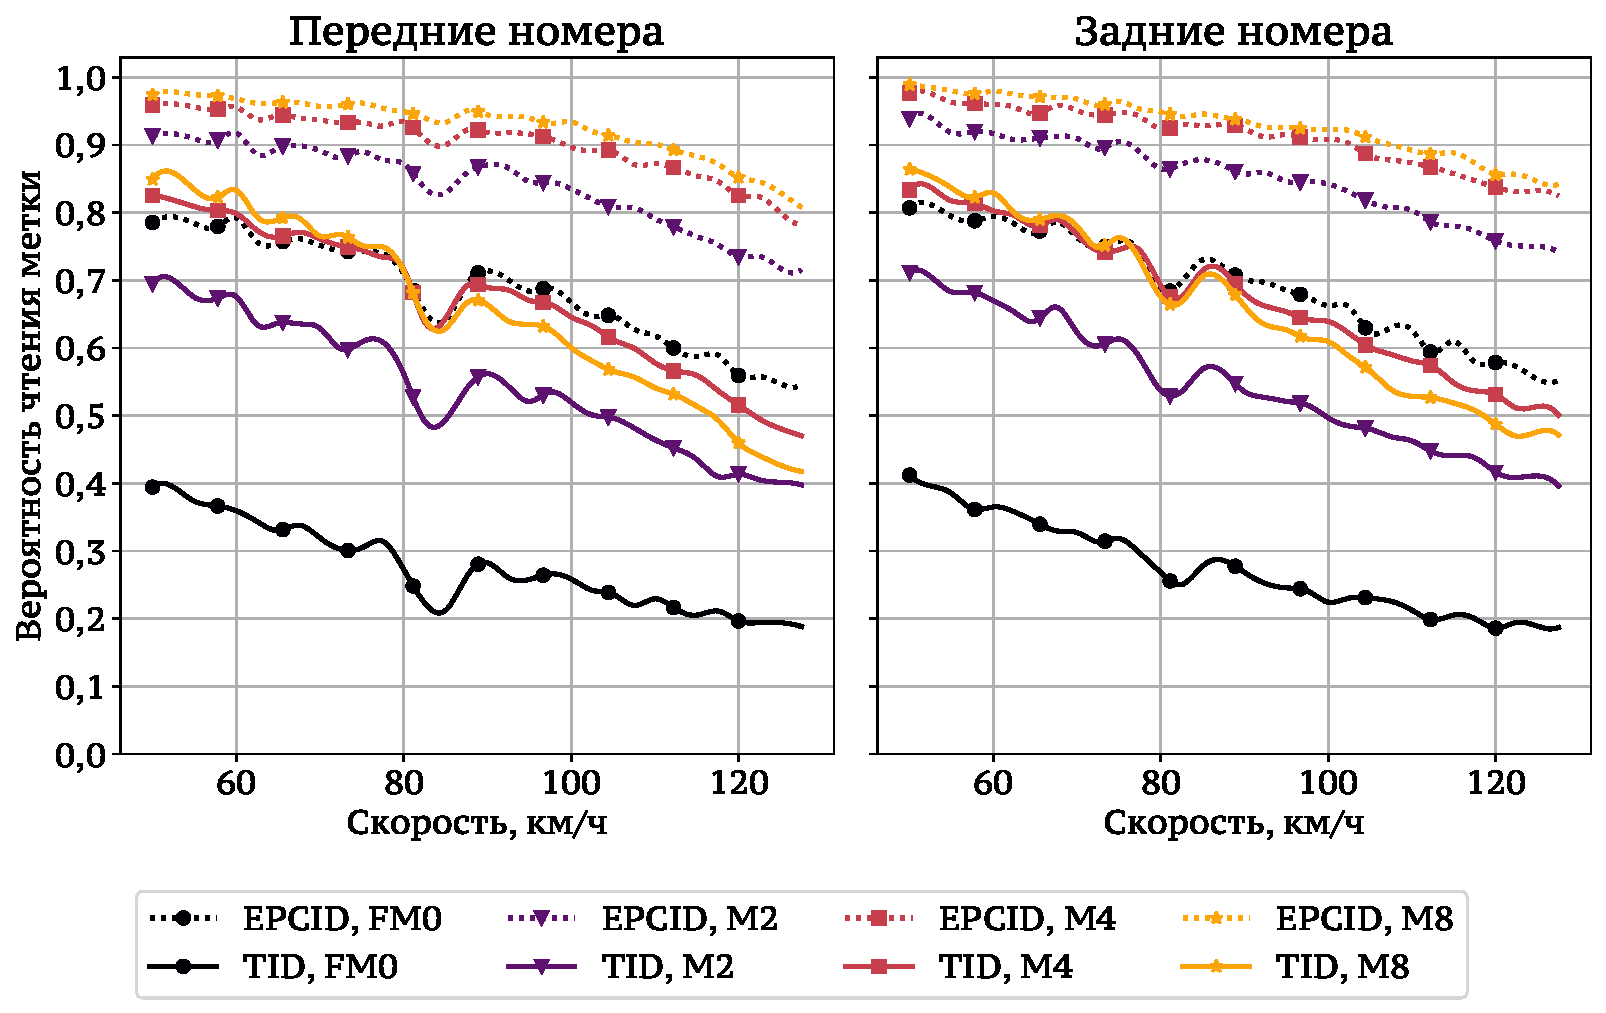
\includegraphics[width=0.8\textwidth]{chapter2/ch2_tag_identification_tari125}
    \end{center}
    \begin{itemize}
        \item При низкой скорости эффективнее использовать код c M = 8 симолов на бит, при высокой "--- M = 2.
        \item При использовании самого быстрого и ненадежного кода FM0 (M = 1) вероятность идентификации слишком низкая.
    \end{itemize}
\end{frame}

\begin{frame}
    \frametitle{Вероятность идентификации автомобиля}
    \begin{center}
        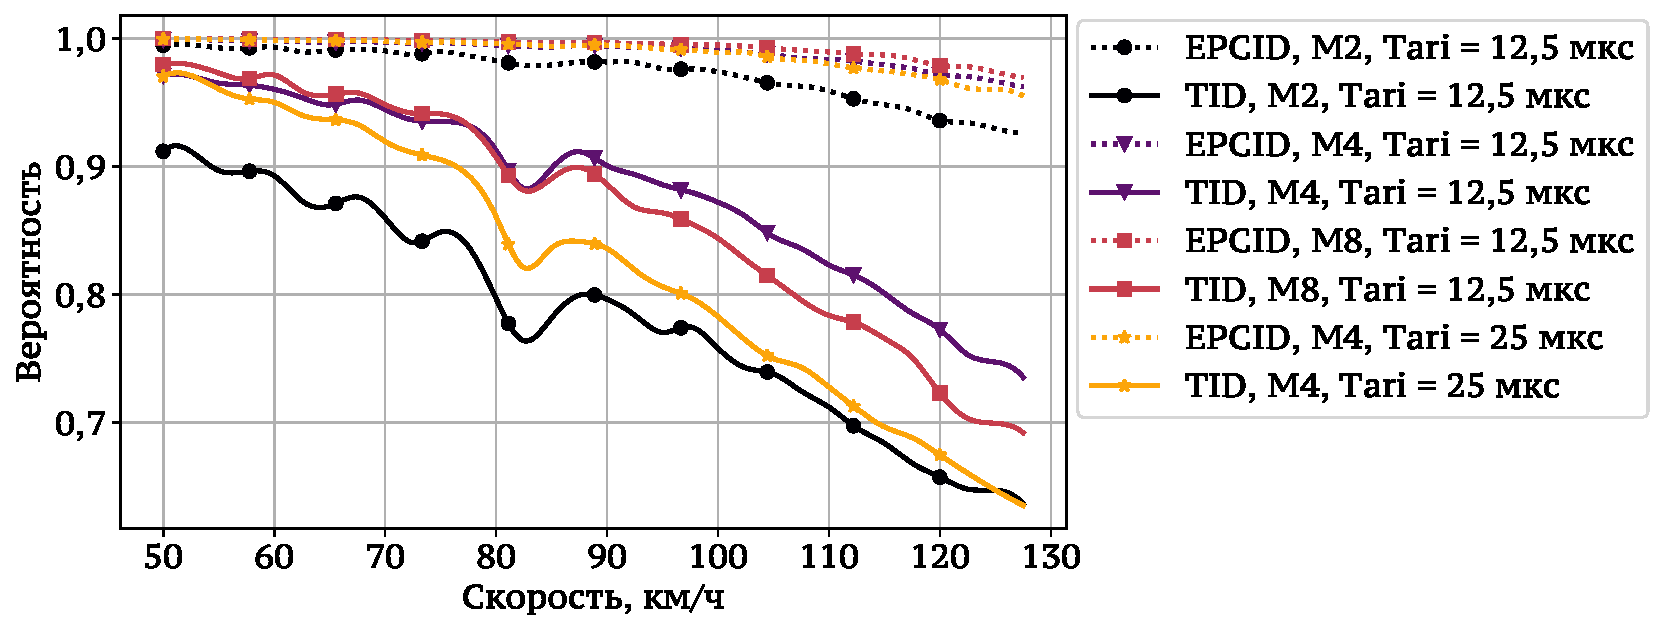
\includegraphics[width=0.85\textwidth]{chapter2/ch2_vehicle_identification_rate}
    \end{center}
    \begin{itemize}
        \item Автомобиль идентифицируется по любой из меток (в переднем или заднем номере).
        \item Самая высокая вероятность идентификации достигается при использовании M = 4 символа на бит в ответах метки и Tari = 12,5~мкс:
        \begin{itemize}
            \item если Tari = 25~мкс или M = 8, раунды опроса становятся слишком длинными;
            \item если M = 1 или M = 2, то вероятность битовой ошибки слишком высока.
        \end{itemize}
    \end{itemize}

\end{frame}

\begin{frame}
    \frametitle{Выводы}
\end{frame}



% ============================================================================
% ЧАСТЬ 3. АНАЛИТИЧЕСКАЯ МОДЕЛЬ СИСТЕМЫ РАДИОЧАСТОТНОЙ ИДЕНТИФИКАЦИИ
% ============================================================================
\section{Аналитическая модель системы радиочастотной идентификации}
\begin{frame}[plain, noframenumbering]
    \begin{center}
        \Huge
        Аналитическая модель системы радиочастотной идентификации
    \end{center}
\end{frame}

\begin{frame}
    \frametitle{Сбросы питания считывателя и флаги сессий в RFID}
\end{frame}

\begin{frame}
    \frametitle{Ограничения и допущения модели}
\end{frame}

\begin{frame}
    \frametitle{Постановка задачи}
\end{frame}

\begin{frame}
    \frametitle{Моделирование раундов инвентаризации}
\end{frame}

\begin{frame}
    \frametitle{Элементарные операции}
\end{frame}

\begin{frame}
    \frametitle{Размеченные сценарии}
\end{frame}

\begin{frame}
    \frametitle{Определение фонового процесса}
\end{frame}

\begin{frame}
    \frametitle{Матрицы операций фнового процесса}
\end{frame}

\begin{frame}
    \frametitle{Расчет распределения числа активных меток}
\end{frame}

\begin{frame}
    \frametitle{Определение основного процесса}
\end{frame}

\begin{frame}
    \frametitle{Матрицы операций основного процесса}
\end{frame}

\begin{frame}
    \frametitle{Расчет вероятности идентификации}
\end{frame}

\begin{frame}
    \frametitle{Результаты: анализ свойств раундов}
\end{frame}

\begin{frame}
    \frametitle{Результаты: валидация модели}
\end{frame}

\begin{frame}
    \frametitle{Результаты: вероятность идентификации}
\end{frame}

\begin{frame}
    \frametitle{Выводы}
\end{frame}





% ============================================================================
% ЧАСТЬ 4. АНАЛИЗ ПРОИЗВОДИТЕЛЬНОСТИ ОПОРНОЙ БЕСПРОВОДНОЙ СЕТИ
% ============================================================================
\section{Анализ производительности опорной беспроводной сети}
\begin{frame}[plain, noframenumbering]
    \begin{center}
        \Huge
        Анализ производительности опорной беспроводной сети
    \end{center}
\end{frame}

\begin{frame}
    \frametitle{Беспроводная сеть передачи данных}
\end{frame}

\begin{frame}
    \frametitle{Моделирование беспроводной сети с помощью СеМО}
\end{frame}

\begin{frame}
    \frametitle{PH-распределения}
\end{frame}

\begin{frame}
    \frametitle{MAP-потоки}
\end{frame}

\begin{frame}
    \frametitle{Многофазные сети с узлами MAP/PH/1/N}
\end{frame}

\begin{frame}
    \frametitle{Итерационный расчет характеристик СеМО}
\end{frame}

\begin{frame}
    \frametitle{Расчет характеристик СеМО методом Монте-Карло}
\end{frame}

\begin{frame}
    \frametitle{Расчет методом понижения размерностей потоков}
\end{frame}

\begin{frame}
    \frametitle{Набор денных для проведения численных исследований}
\end{frame}

\begin{frame}
    \frametitle{Аппроксимация потоков по среднему значению}
\end{frame}

\begin{frame}
    \frametitle{Аппроксимация PH по двум моментам}
\end{frame}

\begin{frame}
    \frametitle{Аппроксимация PH по трем моментам}
\end{frame}

\begin{frame}
    \frametitle{Аппроксимация MAP по трем моментам и корреляции}
\end{frame}

\begin{frame}
    \frametitle{Сравнение эффективности методов аппроксимации}
\end{frame}

\begin{frame}
    \frametitle{Длительность передачи пакета в IEEE 802.11}
\end{frame}

\begin{frame}
    \frametitle{Калибровочная беспроводная сеть}
\end{frame}

\begin{frame}
    \frametitle{Методика: выбор PH-распределений для модели сети}
\end{frame}

\begin{frame}
    \frametitle{Имитационное моделирование беспроводной сети}
\end{frame}

\begin{frame}
    \frametitle{Характеристики каналов калибровочной сети}
\end{frame}

\begin{frame}
    \frametitle{Валидация модели по калибровочной сети}
\end{frame}

\begin{frame}
    \frametitle{Межконцевые задержки в сетях проивзольного размера}
\end{frame}

\begin{frame}
    \frametitle{Изменение задержек в каналах}
\end{frame}

\begin{frame}
    \frametitle{Обновленная методика выбора распределений}
\end{frame}

\begin{frame}
    \frametitle{Межконцевые задержки (обновленная методика)}
\end{frame}

\begin{frame}
    \frametitle{Ошибки в оценке задержек}
\end{frame}

\begin{frame}
    \frametitle{Выводы}
\end{frame}


% ============================================================================
% ЧАСТЬ 5. РАЗРАБОТКА И ЭКСПЕРИМЕНТАЛЬНОЕ ВНЕДРЕНИЕ СИСТЕМЫ РАДИОЧАСТОТНОЙ
%          ИДЕНТИФИКАЦИИ
% ============================================================================
\section{Разработка и экспериментальное внедрение системы радиочастотной идентификации}
\begin{frame}[plain, noframenumbering]
    \begin{center}
        \Huge
        Разработка и экспериментальное внедрение системы радиочастотной идентификации
    \end{center}
\end{frame}

\begin{frame}
    \frametitle{Постановка задачи}
\end{frame}

\begin{frame}
    \frametitle{Архитектура распределенной системы}
\end{frame}

\begin{frame}
    \frametitle{Основные компоненты системы}
\end{frame}

\begin{frame}
    \frametitle{Способы размещения компонентов}
\end{frame}

\begin{frame}
    \frametitle{Протоколы связи между компонентами}
\end{frame}

\begin{frame}
    \frametitle{Протокол управления компонентами IMMP}
\end{frame}

\begin{frame}
    \frametitle{Протокол работы с RFID-адаптерами ITOP}
\end{frame}

\begin{frame}
    \frametitle{Протокол подключения абонентов TFP}
\end{frame}

\begin{frame}
    \frametitle{Протокол подключения интерфейсов SUAP}
\end{frame}

\begin{frame}
    \frametitle{Организация параллельной обработки}
\end{frame}

\begin{frame}
    \frametitle{Особенности реализации системы}
\end{frame}

\begin{frame}
    \frametitle{Структура RFID-считывателя}
\end{frame}

\begin{frame}
    \frametitle{Эксперимент №1: Казань, 2014 год}
\end{frame}

\begin{frame}
    \frametitle{Эксперимент №2: Казань, 2020 год}
\end{frame}

\begin{frame}
    \frametitle{Эксперимент №3: ЦКАД, 2021 год}
\end{frame}

\begin{frame}
    \frametitle{Выводы}
\end{frame}

% % ============================================================================
% % ЧАСТЬ 6. ЗАКЛЮЧЕНИЕ
% % ============================================================================
% \section{Заключение}



% ============================================================================
% ЧАСТЬ -. ПРИМЕРЫ
% ============================================================================
\section{-- Примеры --}
\begin{frame}[plain, noframenumbering]
    \begin{center}
        \Huge
        ПРИМЕРЫ ИЗ ПАКЕТА PHD-THESIS-LATEX
    \end{center}
\end{frame}
\begin{frame}[plain, noframenumbering]
    \begin{center}
        \Huge
        Графика
    \end{center}
\end{frame}


\begin{frame}[plain, noframenumbering]
    \frametitle{Одиночное изображение}
    \centering
    \includegraphics[width=0.8\linewidth]{latex} % окружение figure не требуется
\end{frame}

\begin{frame}[plain, noframenumbering]
    \frametitle{Векторная графика}
    \begin{figure}
	    \centering
	    \ifdefmacro{\tikzsetnextfilename}{\tikzsetnextfilename{tikz_presentation}}{}% присваиваемое предкомпилированному pdf имя файла (не обязательно)
	    \input{Presentation/images/tikz_plot.tikz}
    \end{figure}
\end{frame}


\begin{frame}[plain, noframenumbering]
    \frametitle{Изображения по-вертикали}
    \centering
    \vfill
    \includegraphics[width=0.8\linewidth,height=0.1\textheight]{latex} \\
    \TeX
    \vfill
    \includegraphics[width=0.8\linewidth,height=0.2\textheight]{latex} \\
    \LaTeX
    \vfill
    \includegraphics[scale=0.2]{latex} \\
    \vfill
\end{frame}


\begin{frame}[plain, noframenumbering]
    \frametitle{Изображения по-горизонтали}
    \begin{minipage}[t]{0.47\linewidth}
        \textbf{Составная \\ подпись 1}
        \center{\includegraphics[width=1\linewidth]{knuth1}}
    \end{minipage}
    \hfill
    \begin{minipage}[t]{0.47\linewidth}
        \textbf{Составная \\ подпись 2}
        \center{\includegraphics[width=1\linewidth]{knuth2}}
    \end{minipage}
\end{frame}

\begin{frame}[plain, noframenumbering]
    \frametitle{Разделяющие линии}
    \begin{minipage}[c]{0.47\linewidth}
        \center{\includegraphics[width=1\linewidth]{latex}}
        \bigskip
        \hrule{}
        \bigskip
        \textbf{Составная \\ подпись 1}
    \end{minipage}
    \hfill
    \vrule{}
    \hfill
    \begin{minipage}[c]{0.47\linewidth}
        \flushright
        \textbf{Составная \\ подпись 2}
        \center{\includegraphics[width=1\linewidth]{knuth2}}
    \end{minipage}
\end{frame}

\begin{frame}[plain, noframenumbering]
    \begin{center}
        \Huge
        Остальное
    \end{center}
\end{frame}


\begin{frame}[plain, noframenumbering]
    \frametitle{Формулы}
    \[
    \left\{
    \begin{array}{rl}
        \dot x = & \sigma (y-x)  \\
        \dot y = & x (r - z) - y \\
        \dot z = & xy - bz
    \end{array}
    \right.
    \]
\end{frame}

\begin{frame}[plain, noframenumbering]
    \frametitle{amsmath}
    \centering
    \begin{minipage}[t]{0.5\linewidth}
        \begin{multline*}
            y = 1 x^1 + 2 x^2 + 3 x^3 + \\ + 4 x^4 + 5 x^5 + \dots
        \end{multline*}
    \end{minipage}
\end{frame}

\begin{frame}[allowframebreaks, noframenumbering]
    \frametitle{Уравнения Максвелла}
    \centering{
        \small
        \def\arraystretch{1.8}%
        \begin{tabular}{ll}
            \toprule
            Интегральная форма                                                                                                                                          & Дифференциальная форма                                                        \\ \midrule
            \(Q_e(t) = \displaystyle\oiint_S \vec D(t) \cdot d\vec{s} = \displaystyle\iiint_V \rho_v(t) dv\)                                                              & \(\nabla \cdot \vec D(t) = \rho_v(t)\)                                          \\
            \(\displaystyle\oiint_S \vec B(t) \cdot d\vec{s} = 0\)                                                                                                        & \(\nabla \cdot \vec B(t) = 0\)                                                  \\
            \(V_{emf}(t) = \displaystyle\oint_L \vec E(t) \cdot d\vec{l}\) = \(- \displaystyle\iint_S \left[\frac{\partial\vec{B}(t)}{\partial t}\right] \cdot d\vec{s}\)   & \(\nabla \times \vec E(t) = - \frac{\partial\vec{B}(t)}{\partial t}\)           \\
            \(I(t) = \displaystyle\oint_L \vec H(t) \cdot d\vec{l} = \displaystyle\iint_S \left[\vec J(t) + \frac{\partial\vec{D}(t)}{\partial t}\right] \cdot d\vec{s}\) & \(\nabla \times \vec H(t) = \vec J(t) + \frac{\partial\vec{D}(t)}{\partial t}\) \\ \midrule
            \(\displaystyle\oiint_S \vec J \cdot d\vec{s} = -\frac{\partial Q_e}{\partial t}\)                                                                            & \(\nabla \cdot \vec J = - \frac{\partial \rho_v}{\partial t}\)                  \\
            \bottomrule
            \multicolumn{2}{c}{\(\vec D(t) = \left[\varepsilon(t)\right] * \vec E(t)\)}                                                                                                                                                                   \\
            \multicolumn{2}{c}{\(\vec B(t) = \left[\mu(t)\right] * \vec H(t)\)}                                                                                                                                                                           \\
        \end{tabular}
    }
    \framebreak

    \hspace{0.05\linewidth}
    \centering{
        \small
        \def\arraystretch{1.8}%
        \begin{tabular}{ll}
            \toprule
            Интегральная форма                                                                                                            & Дифференциальная форма                             \\ \midrule
            \(Q_e = \displaystyle\oiint_S \vec D \cdot d\vec{s} = \displaystyle\iiint_V \rho_v dv\)                                         & \(\nabla \cdot \vec D = \rho_v\)                     \\
            \(\displaystyle\oiint_S \vec B \cdot d\vec{s} = 0\)                                                                             & \(\nabla \cdot \vec B = 0\)                          \\
            \(V_{emf} = \displaystyle\oint_L \vec E \cdot d\vec{l}\) = \(- \displaystyle\iint_S \left[j \omega \vec B\right] \cdot d\vec{s}\) & \(\nabla \times \vec E = - j \omega \vec B\)         \\
            \(I = \displaystyle\oint_L \vec H \cdot d\vec{l} = \displaystyle\iint_S \left[\vec J + j \omega \vec D\right] \cdot d\vec{s}\)  & \(\nabla \times \vec H = \vec J + j \omega \vec{D}\) \\ \midrule
            \(\displaystyle\oiint_S \vec J \cdot d\vec{s} = - j \omega Q_e\)                                                                & \(\nabla \cdot \vec J = - j \omega \rho_v\)          \\
            \bottomrule
            \multicolumn{2}{c}{\(\vec D(t) = \left[\varepsilon\right] \vec E(t)\)}                                                                                                               \\
            \multicolumn{2}{c}{\(\vec B(t) = \left[\mu\right] \vec H(t)\)}                                                                                                                       \\
        \end{tabular}
    }
\end{frame}

\begin{frame}[plain, noframenumbering]
    \frametitle{Таблица}
    \centering
    \begin{tabular}{|l|l|}
        \hline
        \textbf{Заголовок 1} & \textbf{Заголовок 2} \\
        \hline
        Сумма                & \(b+a\)                \\
        \hline
        Разность             & \(a-b\)                \\
        \hline
        Произведение         & \(a*b\)                \\
        \hline
    \end{tabular}
\end{frame}

\begin{frame}[plain, noframenumbering]
    \frametitle{Другая таблица}
    \centering
    \begin{tabular}{lc}
        \toprule
        \multicolumn{1}{c}{\textbf{Заголовок 1}} & \textbf{Заголовок 2} \\ \midrule
        Сумма                                    & \(b+a\)                \\
        Разность                                 & \(a-b\)                \\
        Произведение                             & \(a*b\)                \\
        \bottomrule
    \end{tabular}
\end{frame}


\begin{frame}[plain, noframenumbering]
    \frametitle{Большой многоуровневый список}
    \begin{itemize}
        \item \textbf{Пункт 1}
              \begin{itemize}
                  \itemi Подпункт 1-1
                  \itemi Подпункт 1-2
              \end{itemize}
        \item \textbf{Пункт 2}
              \begin{itemize}
                  \itemi Подпункт 2-1
              \end{itemize}
        \item \textbf{Пункт 3}
              \begin{itemize}
                  \itemi Подпункт 3-1
                  \itemi Подпункт 3-2
              \end{itemize}
        \item \textbf{Пункт 4}
              \begin{itemize}
                  \itemi Подпункт 4-1
              \end{itemize}
        \item \textbf{Пункт 5}
              \begin{itemize}
                  \itemi Подпункт 5-1
                  \itemi Подпункт 5-2
                  \itemi Подпункт 5-3
              \end{itemize}
    \end{itemize}
\end{frame}

\begin{frame}[plain, noframenumbering]
    \frametitle{Четыре изображения}
    \centering
    \includegraphics[width=0.35\linewidth,angle=35]{latex}
    \includegraphics[width=0.35\linewidth,angle=135]{latex}\\
    \includegraphics[width=0.35\linewidth,angle=15]{latex}
    \includegraphics[width=0.35\linewidth,angle=-15]{latex}
\end{frame}

\begin{frame}[allowframebreaks]
    \frametitle{Списки}
    \begin{itemize}
        \item Проблема 1
        \item Проблема 2
        \item Проблема 3
    \end{itemize}
    \framebreak
    \begin{enumerate}
        \item \textbf{Задача 1}
              \begin{itemize}
                  \item Подзадача 1-1
                  \item Подзадача 1-2
              \end{itemize}
        \item \textbf{Задача 2}
              \begin{itemize}
                  \item Подзадача 2-1
                  \item Подзадача 2-2
                  \item Подзадача 2-3
              \end{itemize}
        \item \textbf{Задача 3}
              \begin{itemize}
                  \item Подзадача 3-1
                  \item Подзадача 3-2
                  \item Подзадача 3-3
              \end{itemize}
    \end{enumerate}
    \framebreak
    Поясняющий текст
    \begin{itemize}
        \item Один
        \item Два
        \item Три
    \end{itemize}
\end{frame}
\note[itemize]{
    \item Тезис 1
    \item Тезис 2
    \item Тезис 3
}
